\documentclass[runningheads]{llncs}

\usepackage{booktabs}
\usepackage{graphicx}
\usepackage{hyperref}
\usepackage{microtype}
\usepackage{url}

\graphicspath{{camera_ready_figures/}}
% Generated from saved evaluation CSV files. Do not edit manually.
\newcommand{\OriginalYoloImageSize}{1280}
\newcommand{\OriginalYoloPrecision}{0.880}
\newcommand{\OriginalYoloRecall}{0.866}
\newcommand{\OriginalYoloFOne}{0.873}
\newcommand{\OriginalYoloMAPFifty}{0.902}
\newcommand{\OriginalYoloMAPStrict}{0.502}
\newcommand{\OriginalYoloInferenceMs}{12.8}
\newcommand{\OriginalYoloTotalMs}{15.2}
\newcommand{\OriginalRTImageSize}{640}
\newcommand{\OriginalRTPrecision}{0.886}
\newcommand{\OriginalRTRecall}{0.839}
\newcommand{\OriginalRTFOne}{0.862}
\newcommand{\OriginalRTMAPFifty}{0.887}
\newcommand{\OriginalRTMAPStrict}{0.470}
\newcommand{\OriginalRTInferenceMs}{48.8}
\newcommand{\OriginalRTTotalMs}{49.8}
\newcommand{\DiagnosticYoloImageSize}{640}
\newcommand{\DiagnosticYoloPrecision}{0.874}
\newcommand{\DiagnosticYoloRecall}{0.810}
\newcommand{\DiagnosticYoloFOne}{0.841}
\newcommand{\DiagnosticYoloMAPFifty}{0.855}
\newcommand{\DiagnosticYoloMAPStrict}{0.453}
\newcommand{\DiagnosticYoloInferenceMs}{12.1}
\newcommand{\DiagnosticYoloTotalMs}{13.8}
\newcommand{\MatchedYoloImageSize}{640}
\newcommand{\MatchedYoloPrecision}{0.870}
\newcommand{\MatchedYoloRecall}{0.852}
\newcommand{\MatchedYoloFOne}{0.861}
\newcommand{\MatchedYoloMAPFifty}{0.892}
\newcommand{\MatchedYoloMAPStrict}{0.482}
\newcommand{\MatchedYoloInferenceMs}{11.4}
\newcommand{\MatchedYoloTotalMs}{13.2}
\newcommand{\MatchedRTImageSize}{640}
\newcommand{\MatchedRTPrecision}{0.867}
\newcommand{\MatchedRTRecall}{0.839}
\newcommand{\MatchedRTFOne}{0.853}
\newcommand{\MatchedRTMAPFifty}{0.881}
\newcommand{\MatchedRTMAPStrict}{0.462}
\newcommand{\MatchedRTInferenceMs}{48.0}
\newcommand{\MatchedRTTotalMs}{49.0}
\newcommand{\HighRTImageSize}{1280}
\newcommand{\HighRTPrecision}{0.766}
\newcommand{\HighRTRecall}{0.534}
\newcommand{\HighRTFOne}{0.630}
\newcommand{\HighRTMAPFifty}{0.604}
\newcommand{\HighRTMAPStrict}{0.295}
\newcommand{\HighRTInferenceMs}{72.4}
\newcommand{\HighRTTotalMs}{74.4}
\newcommand{\MatchedRecallDelta}{0.013}
\newcommand{\MatchedMAPStrictDelta}{0.020}


\begin{document}

\title{Real-Time PCB Defect Detection for Embedded Visual Inspection:
A Same-Split Comparison of YOLO11s and RT-DETR-L}

\titlerunning{Resolution-Controlled PCB Defect Detection}

\author{Aditya Varun Dhayapulay\inst{1}
\and Paul Salvador Inventado\inst{1}}

\authorrunning{A. V. Dhayapulay and P. S. Inventado}

\institute{California State University, Fullerton, Fullerton, CA, USA\\
\email{adivd@csu.fullerton.edu; pinventado@fullerton.edu}}

\maketitle

\begin{abstract}
Printed circuit board inspection requires reliable localization of small
defects at latency compatible with manufacturing workflows. We compare
YOLO11s and RT-DETR-L on one 5,551/1,016/1,016 train, validation, and
test split covering six PCB defect classes. The accepted practical
configurations use YOLO11s at 1280 pixels and RT-DETR-L at 640 pixels.
To separate architecture effects from input-resolution effects, the
camera-ready study adds models trained and evaluated at a matched
640-pixel resolution under an identical batch-1, no-test-time-augmentation
protocol on NVIDIA Tesla V100-SXM2-32GB hardware. At 640 pixels,
YOLO11s obtains \MatchedYoloRecall{} recall and
\MatchedYoloMAPStrict{} mAP50--95, while RT-DETR-L obtains
\MatchedRTRecall{} recall and \MatchedRTMAPStrict{} mAP50--95.
We also report RT-DETR-L at \HighRTImageSize{} pixels, per-class results,
and representative success and failure cases. The study contributes a
reproducible, deployment-oriented benchmark rather than a new detector
architecture. A browser-based inference demo is provided as an online
deployment artifact; embedded-device and TensorRT benchmarking remain
future work.

\keywords{PCB defect detection \and embedded vision \and YOLO11
\and RT-DETR \and object detection \and industrial inspection}
\end{abstract}

\section{Introduction}

Printed circuit boards (PCBs) are central to embedded and cyber-physical
products. A missing hole, short, copper spur, or other visual defect on
an unpopulated board can become substantially more expensive after
assembly. Automated optical inspection is therefore not only an
accuracy problem: a detector must find small defects, localize them
well enough for review or repair, and execute within the timing and
resource constraints of an inspection workflow.

This paper studies six defect classes: Missing\_hole, Mouse\_bite,
Open\_circuit, Short, Spur, and Spurious\_copper. The accepted
submission compared a completed YOLO11s model trained at 1280 pixels
with a completed RT-DETR-L model trained at 640 pixels. Both checkpoints
used the same dataset split and evaluator, but the input-size difference
meant that the result was a comparison of practical completed
configurations rather than a controlled architecture-only ablation.

The camera-ready study preserves that practical comparison and adds
the following:

\begin{itemize}
\item a matched-resolution YOLO11s-640 versus RT-DETR-L-640 experiment;
\item a completed RT-DETR-L high-resolution experiment at 1280 pixels
and batch size 1, which did not require the planned 960-pixel fallback;
\item a corrected canonical class-ID mapping for semantic per-class
analysis;
\item class-balanced detection examples and representative failure
cases; and
\item a complete manifest connecting dataset counts, software versions,
hardware, seeds, checkpoints, tables, and figures.
\end{itemize}

The contribution is a traceable benchmark for choosing a practical
PCB inspection baseline. We do not claim a new architecture or
embedded-device performance.

\section{Related Work}

PCB defect inspection has progressed from reference-image comparison
and rule-based machine vision to learned object detectors. Classical
systems can be efficient when board registration, lighting, and product
geometry are tightly controlled, but they often require product-specific
thresholds and feature engineering. Learned detectors jointly classify
and localize a defect, which is useful when the output feeds human
review, repair guidance, or process analytics. The six-class PCB
dataset introduced by Huang and Wei is a common reference for this
problem~\cite{huang2019pcb}.

YOLO-family detectors are widely used when latency matters because they
predict classes and boxes in one forward pass. We use Ultralytics
YOLO11s~\cite{ultralytics2026yolo11} as the compact convolutional
baseline. RT-DETR~\cite{zhao2024rtdetr} provides a contrasting
transformer-style design intended for real-time end-to-end detection.
The comparison is useful for PCB inspection because small, sparse
defects stress both feature resolution and bounding-box precision.

Detector fusion can increase recall when missed defects are more costly
than false alarms. The accepted study included Weighted Boxes Fusion
(WBF)~\cite{solovyev2021wbf} as supporting analysis. The present
resolution-control experiment focuses on single-model comparisons so
that resolution and architecture effects remain interpretable.

\section{Dataset and Experimental Protocol}

\subsection{Dataset}

The primary corpus, denoted \texttt{YOLO\_PCB}, combines the project
PCB dataset with overlapping classes from DsPCBSD+~\cite{dspcbsdplus}.
The deterministic preparation procedure uses seed 42, stratifies within
source/class groups, and produces 5,551 training, 1,016 validation, and
1,016 test images. The validation partition contains 2,106 annotated
instances and the test partition contains 2,179. The training split
includes 800 class-balancing copy-paste images: 320 Missing\_hole,
240 Mouse\_bite, and 240 Spur examples.

\begin{table}
\caption{Canonical defect classes used by the controlled experiments.}
\label{tab:classes}
\centering
\begin{tabular}{cl}
\toprule
ID & Class\\
\midrule
0 & Missing\_hole\\
1 & Mouse\_bite\\
2 & Open\_circuit\\
3 & Short\\
4 & Spur\\
5 & Spurious\_copper\\
\bottomrule
\end{tabular}
\end{table}

A reproducibility audit found that an earlier dataset export changed
the displayed class-name order without remapping label IDs. This does
not change class-agnostic aggregate precision, recall, or mAP, but it
can misname per-class rows. We therefore use two explicit dataset
manifests: a legacy ID layout solely for reproducing the accepted
aggregate baselines, and the canonical semantic mapping in
Table~\ref{tab:classes} for all new training and per-class claims.
Both manifests contain identical image assignments and instance counts.

\subsection{Models and Training}

The original YOLO11s checkpoint was trained for 50 epochs at 1280 pixels
with batch size 12. The original RT-DETR-L checkpoint was trained for
10 epochs at 640 pixels with batch size 4. These checkpoints are
preserved unchanged.

For the controlled study, YOLO11s is trained for 50 epochs at 640 pixels
with batch size 12 and seed 42. RT-DETR-L is trained for 10 epochs at
640 pixels with batch size 4 and seed 42. The high-resolution
RT-DETR-L run uses 10 epochs, batch size 1, and seed 42 at
\HighRTImageSize{} pixels. A one-epoch smoke test precedes every full
training configuration. The 1280-pixel run completed successfully, so
the planned 960-pixel out-of-memory fallback was not used.

\subsection{Evaluation}

Every reported model is evaluated with Ultralytics 8.4.51 and PyTorch
2.5.1 on a Tesla V100-SXM2-32GB. Evaluation uses batch size 1, zero
dataloader workers, the same validation and test images, and no
test-time augmentation. We report precision, recall, F1, mAP50,
mAP50--95, and per-image preprocess, inference, postprocess, and total
latency. Precision is the true-positive fraction among predictions,
recall is the true-positive fraction among labeled instances, and F1 is
their harmonic mean, consistent with the evaluator documentation
used by the pipeline~\cite{ultralytics2026metrics}. The mAP50--95
convention averages average precision over IoU
thresholds from 0.50 to 0.95 in increments of 0.05, following the
COCO evaluation convention~\cite{lin2014coco}.

Before new training begins, the archived checkpoints are evaluated on
the rebuilt legacy split. The pipeline stops if precision, recall,
mAP50, or mAP50--95 differs from the archived value by more than 0.001.
The observed differences were approximately $10^{-8}$, confirming exact
split and evaluator reproduction.

\section{Results}

\subsection{Accepted Practical Configurations}

Table~\ref{tab:practical-test} preserves the accepted comparison. It
should be interpreted as a practical-configuration result:
YOLO11s-1280 versus RT-DETR-L-640, not an input-size-controlled
architecture comparison.

\begin{table*}
\caption{Accepted practical configurations on the test split. All values
are generated from the archived-checkpoint evaluation CSV.}
\label{tab:practical-test}
\centering
\small
\begin{tabular}{lrrrrrrr}
\hline
Model & P & R & F1 & mAP50 & mAP50--95 & Infer. ms & Total ms \\
\hline
YOLO11s 1280 & 0.880 & 0.866 & 0.873 & 0.902 & 0.502 & 12.8 & 15.2 \\
RT-DETR-L 640 & 0.886 & 0.839 & 0.862 & 0.887 & 0.470 & 48.8 & 49.8 \\
\hline
\end{tabular}

\end{table*}

The evaluation-only diagnostic changes the original YOLO11s checkpoint
input size from 1280 to 640 without retraining. Its test recall falls
from \OriginalYoloRecall{} to \DiagnosticYoloRecall{} and mAP50--95
falls from \OriginalYoloMAPStrict{} to \DiagnosticYoloMAPStrict{}.
This result is not the matched comparison; it demonstrates why simply
resizing a checkpoint cannot replace resolution-specific training.

\subsection{Matched Resolution and High-Resolution RT-DETR}

Table~\ref{tab:controlled-test} reports the controlled experiments.
YOLO11s-640 and RT-DETR-L-640 use identical image assignments,
resolution, evaluation batch size, evaluator, hardware class, and
test-time augmentation setting. The matched recall difference
(YOLO11s minus RT-DETR-L) is \MatchedRecallDelta{}, and the matched
mAP50--95 difference is \MatchedMAPStrictDelta{}.

\begin{table*}
\caption{Resolution-controlled and high-resolution configurations on
the test split. Values are generated from the saved evaluation CSV.}
\label{tab:controlled-test}
\centering
\small
\begin{tabular}{lrrrrrrr}
\hline
Model & P & R & F1 & mAP50 & mAP50--95 & Infer. ms & Total ms \\
\hline
RT-DETR-L 640 & 0.867 & 0.839 & 0.853 & 0.881 & 0.462 & 48.0 & 49.0 \\
RT-DETR-L 1280 & 0.766 & 0.534 & 0.630 & 0.604 & 0.295 & 72.4 & 74.4 \\
YOLO11s 640 & 0.870 & 0.852 & 0.861 & 0.892 & 0.482 & 11.4 & 13.2 \\
\hline
\end{tabular}

\end{table*}

The high-resolution RT-DETR-L row is reported separately because it
changes both input size and computational cost. It answers whether the
transformer model benefits from additional spatial detail, but it is
not a replacement for the matched 640-pixel comparison.
In this run, increasing RT-DETR-L to \HighRTImageSize{} pixels did not
improve the measured configuration: test mAP50--95 changed from
\MatchedRTMAPStrict{} at 640 pixels to \HighRTMAPStrict{}, while total
latency increased from \MatchedRTTotalMs{} to \HighRTTotalMs{} ms.
This result suggests that additional pixels alone do not compensate for
the fixed 10-epoch schedule and substantially higher computational cost.

\subsection{Per-Class Behavior}

Table~\ref{tab:per-class} uses only models trained with the corrected
canonical label mapping. It therefore replaces semantic per-class
claims from the accepted draft while leaving the accepted aggregate
baseline unchanged.

\begin{table*}
\caption{Matched 640-pixel per-class test results using canonical labels.}
\label{tab:per-class}
\centering
\scriptsize
\begin{tabular}{llrrrr}
\hline
Class & Model & P & R & mAP50 & mAP50--95 \\
\hline
Missing\_hole & YOLO11s 640 & 0.990 & 0.986 & 0.994 & 0.569 \\
Missing\_hole & RT-DETR-L 640 & 0.962 & 1.000 & 0.995 & 0.567 \\
Mouse\_bite & YOLO11s 640 & 0.821 & 0.763 & 0.835 & 0.403 \\
Mouse\_bite & RT-DETR-L 640 & 0.818 & 0.765 & 0.829 & 0.403 \\
Open\_circuit & YOLO11s 640 & 0.848 & 0.850 & 0.890 & 0.525 \\
Open\_circuit & RT-DETR-L 640 & 0.882 & 0.880 & 0.917 & 0.513 \\
Short & YOLO11s 640 & 0.880 & 0.892 & 0.942 & 0.551 \\
Short & RT-DETR-L 640 & 0.881 & 0.865 & 0.900 & 0.505 \\
Spur & YOLO11s 640 & 0.869 & 0.767 & 0.839 & 0.381 \\
Spur & RT-DETR-L 640 & 0.818 & 0.729 & 0.794 & 0.342 \\
Spurious\_copper & YOLO11s 640 & 0.815 & 0.853 & 0.852 & 0.462 \\
Spurious\_copper & RT-DETR-L 640 & 0.844 & 0.795 & 0.852 & 0.443 \\
\hline
\end{tabular}

\end{table*}

\subsection{Representative Predictions}

The prediction audit matches detections to ground truth at IoU 0.50.
Figure~\ref{fig:successes} selects one successful example per class
where available. Figure~\ref{fig:failures} ranks examples by a
miss-weighted error score, $5FN+FP$, and favors class diversity. The
selection manifest records every source image, ground-truth count,
prediction count, true positive, false positive, and false negative.

\begin{figure}
\centering
\IfFileExists{camera_ready_figures/class_balanced_success_examples.png}
{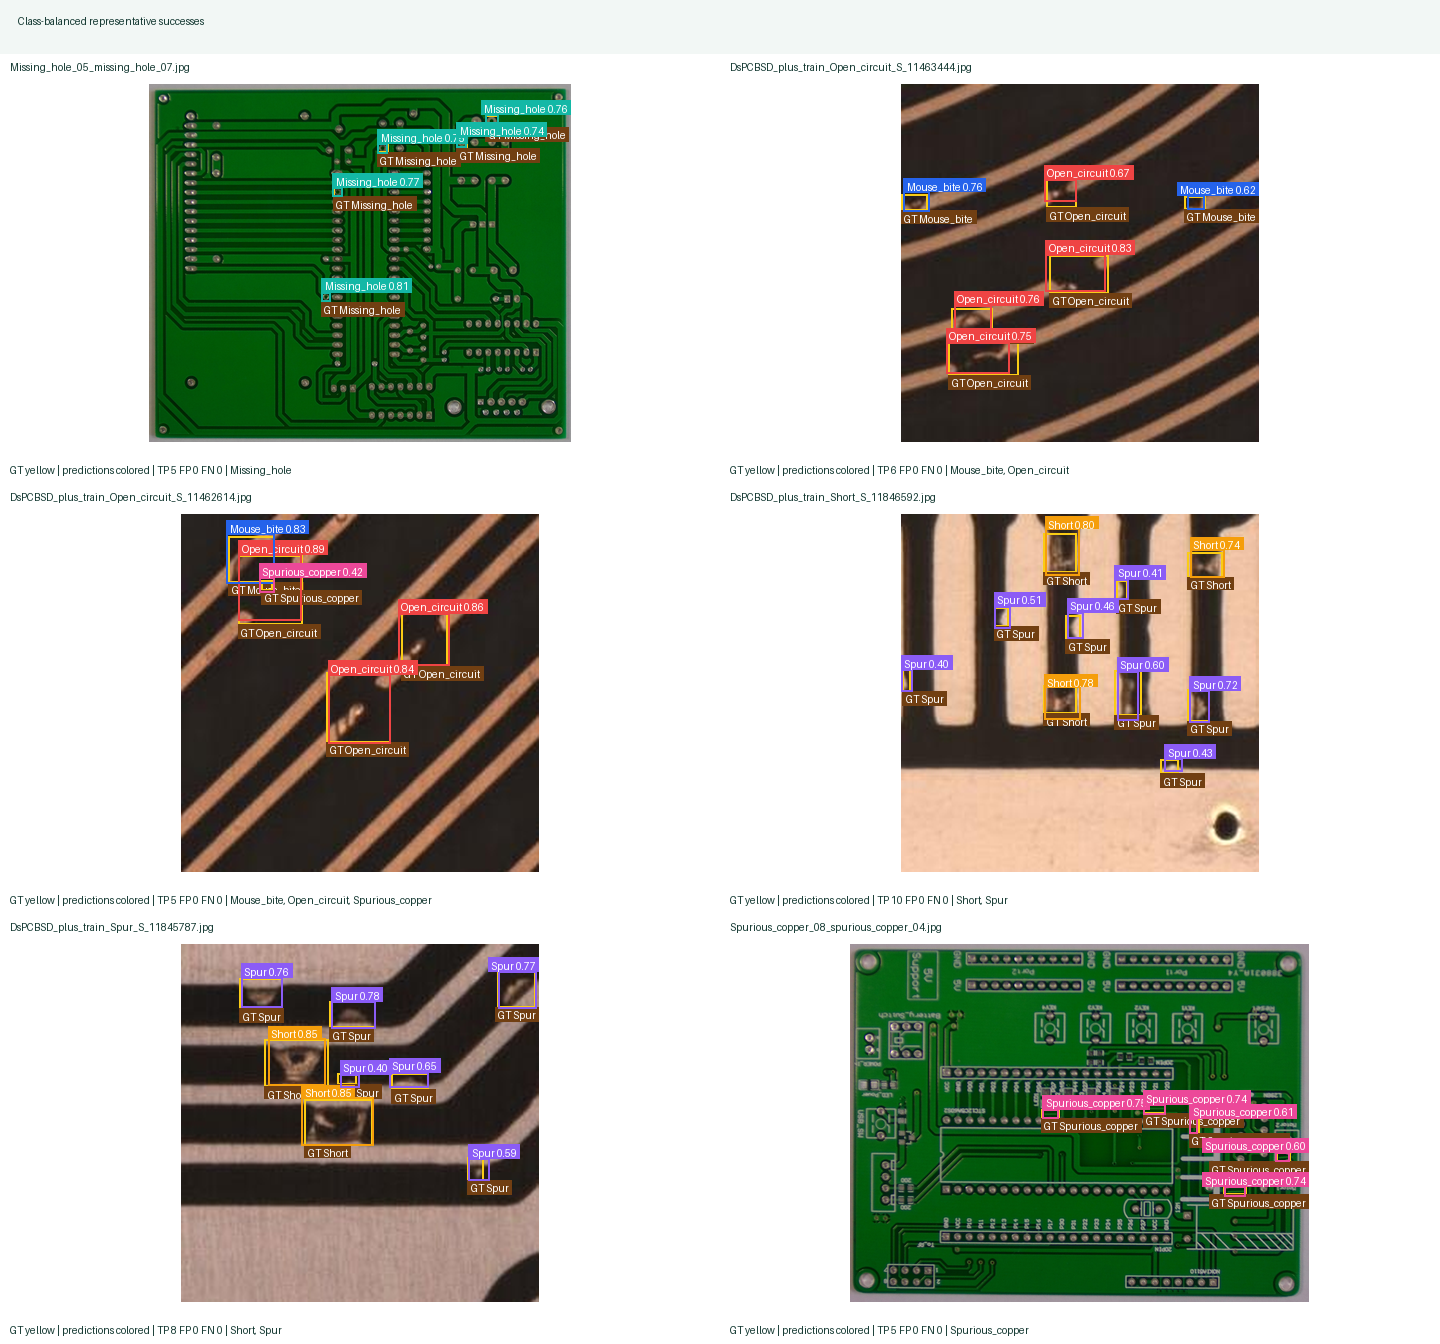
\includegraphics[width=\textwidth]{class_balanced_success_examples.png}}
{\fbox{\parbox{0.9\textwidth}{Class-balanced success figure unavailable.}}}
\caption{Class-balanced representative detections from the matched
YOLO11s-640 test run.}
\label{fig:successes}
\end{figure}

\begin{figure}
\centering
\IfFileExists{camera_ready_figures/representative_failure_cases.png}
{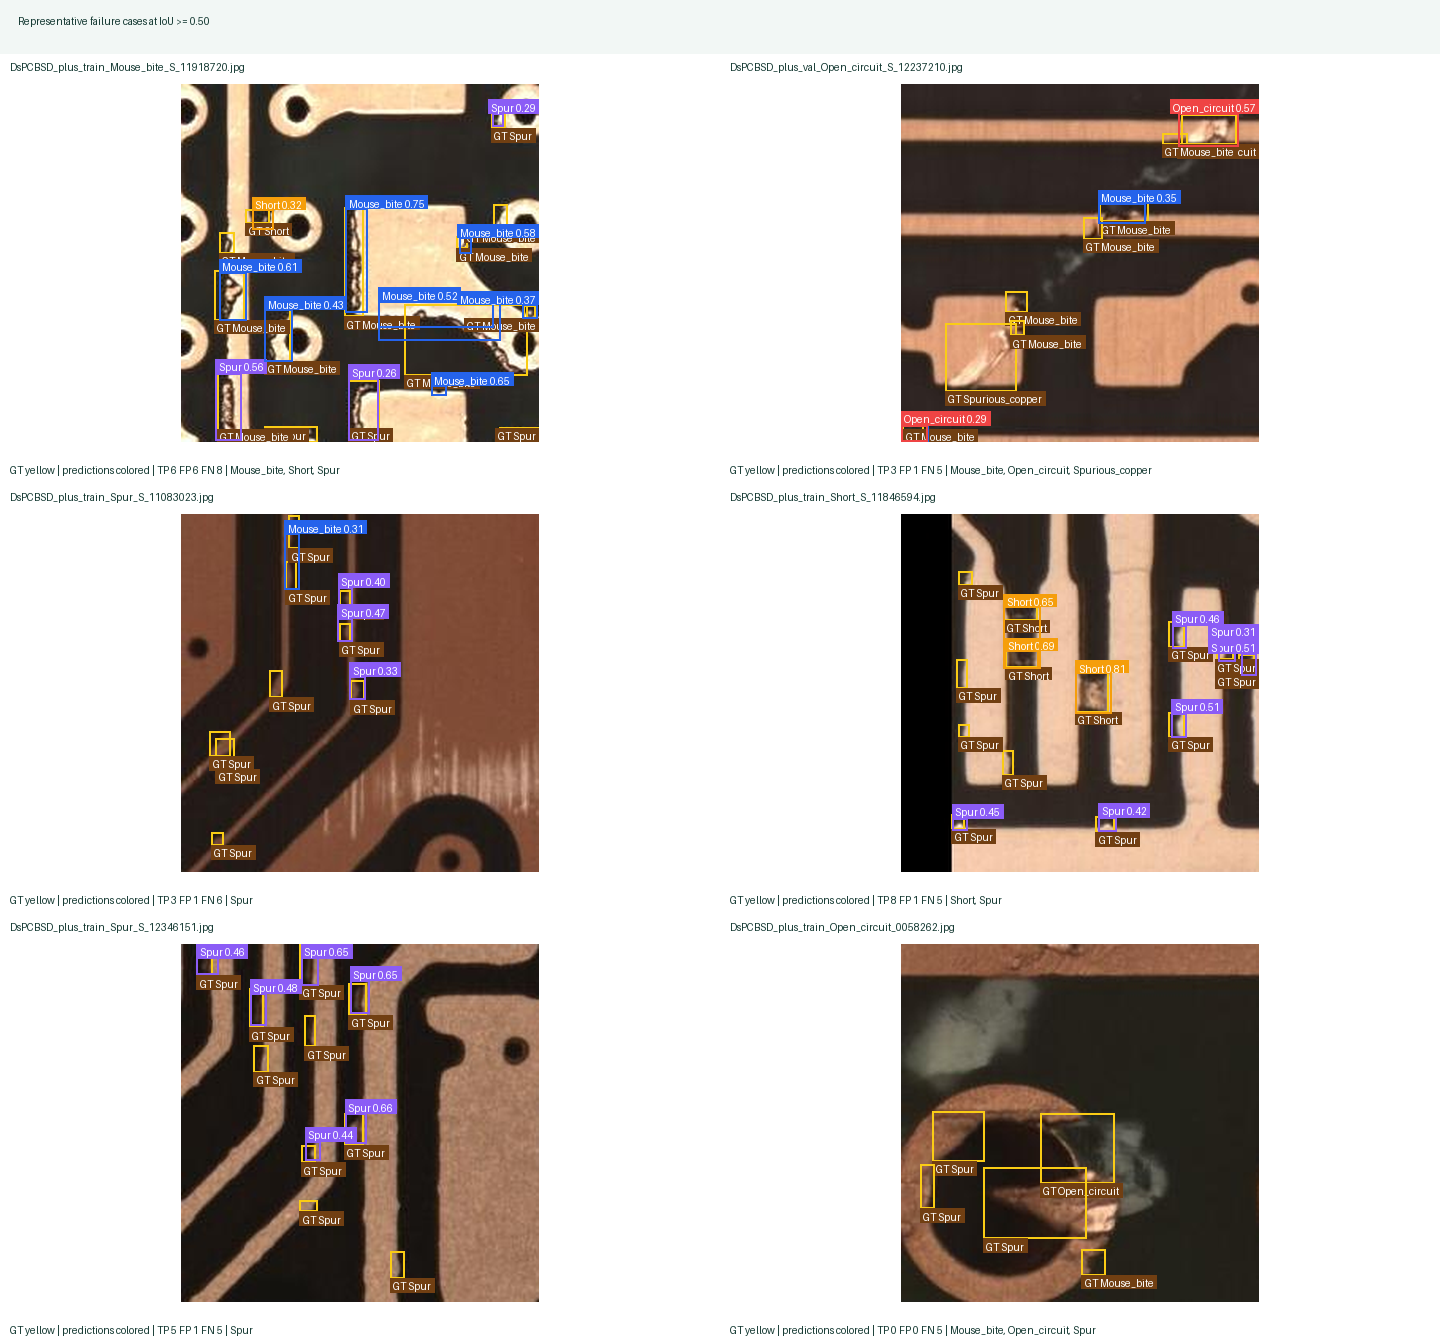
\includegraphics[width=\textwidth]{representative_failure_cases.png}}
{\fbox{\parbox{0.9\textwidth}{Failure-analysis figure unavailable.}}}
\caption{Representative failure cases selected by false-negative and
false-positive counts at IoU 0.50.}
\label{fig:failures}
\end{figure}

\clearpage

\section{Discussion}

The original practical comparison favored YOLO11s-1280 on recall,
strict localization, and latency while RT-DETR-L-640 had a small
precision advantage. Because the configurations used different input
sizes, those results support a deployment choice among completed models,
not a clean architectural ranking.

The matched 640-pixel experiment directly addresses that limitation.
Its interpretation should focus on the direction and magnitude of the
precision, recall, mAP, and latency differences under controlled input
resolution. The high-resolution RT-DETR-L experiment then shows whether
additional spatial detail closes any localization gap and what latency
cost accompanies it. Together, the two tables distinguish resolution
effects from architecture effects more clearly than either experiment
alone.

The matched-resolution study is not a resource-normalized architecture
benchmark. It preserves the completed per-model training schedules:
50 epochs and batch size 12 for YOLO11s, compared with 10 epochs and
batch size 4 for RT-DETR-L. The models also differ in parameter count,
optimization behavior, and computational cost. A claim about detector
architecture alone would require equalized training compute, latency,
memory, FLOPs, or a broader hyperparameter study. We therefore limit
the conclusion to the measured configurations.

The gap between mAP50 and mAP50--95 remains important for inspection.
A model may identify the correct defect region at IoU 0.50 while still
placing a loose box at stricter thresholds. Better localization may
require high-resolution crops, label review, class-specific
augmentation, or a second-stage refinement model rather than only a
larger detector.

\section{Deployment Scope and Limitations}

The trained YOLO checkpoint is served through a public Hugging Face
Space at
\url{https://adiivd-pcb-defect-detection.hf.space}. The browser
workflow accepts an uploaded PCB image and returns annotated detections,
class counts, confidence values, and downloadable results. This is an
online deployment artifact and usability demonstration, not an
embedded-device benchmark.

All latency values in this paper are V100 measurements. We have not
measured either detector on Jetson, TensorRT, RK3588, FPGA, or another
edge-oriented target. We therefore make no claim about target-device
latency, throughput, energy, or memory. The dataset is also an
in-distribution benchmark rather than a factory-domain generalization
study. Lighting variation, registration error, product changes, and
real manufacturing noise require separate validation.

\section{Conclusion}

This work preserves the accepted YOLO11s-1280 versus RT-DETR-L-640
practical comparison and adds the matched-resolution evidence requested
by reviewers. The controlled pipeline uses one split, canonical labels,
pinned V100 hardware, batch-1 evaluation, no TTA, saved CSV tables,
per-class metrics, prediction figures, and an auditable manifest.
The results support a more careful distinction between architecture
and resolution effects while retaining the deployment-oriented goal of
the original study. Future work will evaluate real factory captures,
resource-normalized training, high-resolution crops, and actual
edge-device deployment. Jetson and TensorRT remain future work until
they can be measured directly.

\section*{Acknowledgments}

We thank Christopher Ryu for support with Nautilus/NRP access and
research computing resources. This work used resources available
through the National Research Platform at the University of California,
San Diego~\cite{weitzel2025nrp}. Cursor and OpenAI Codex were used as
programming assistants for code navigation, reproducibility checks,
and manuscript proofreading. The authors reviewed all suggestions and
remain responsible for the experiments, analysis, code, figures, and
text.

\bibliographystyle{splncs04}
\bibliography{escs26_references}

\end{document}
